\chapter{Handout 9}

\emph{Lo que queda de la vieja iglesia se alza al final de una calle torcida y
lúgubre. Las ruinas están tan desgastadas y cubiertas de vegetación que los
escombros de piedra gris parecen más una roca natural que antiguos muros y
cimientos. Pasas junto a un muro desplomado que ostenta símbolos pintados de
blanco, aparentemente recién trazados: tres letras Y dispuestas en un triángulo
de tal manera que los elementos superiores de cada Y tocan a las otras dos. En
el centro, así creado, está pintado un ojo que mira fijamente.}

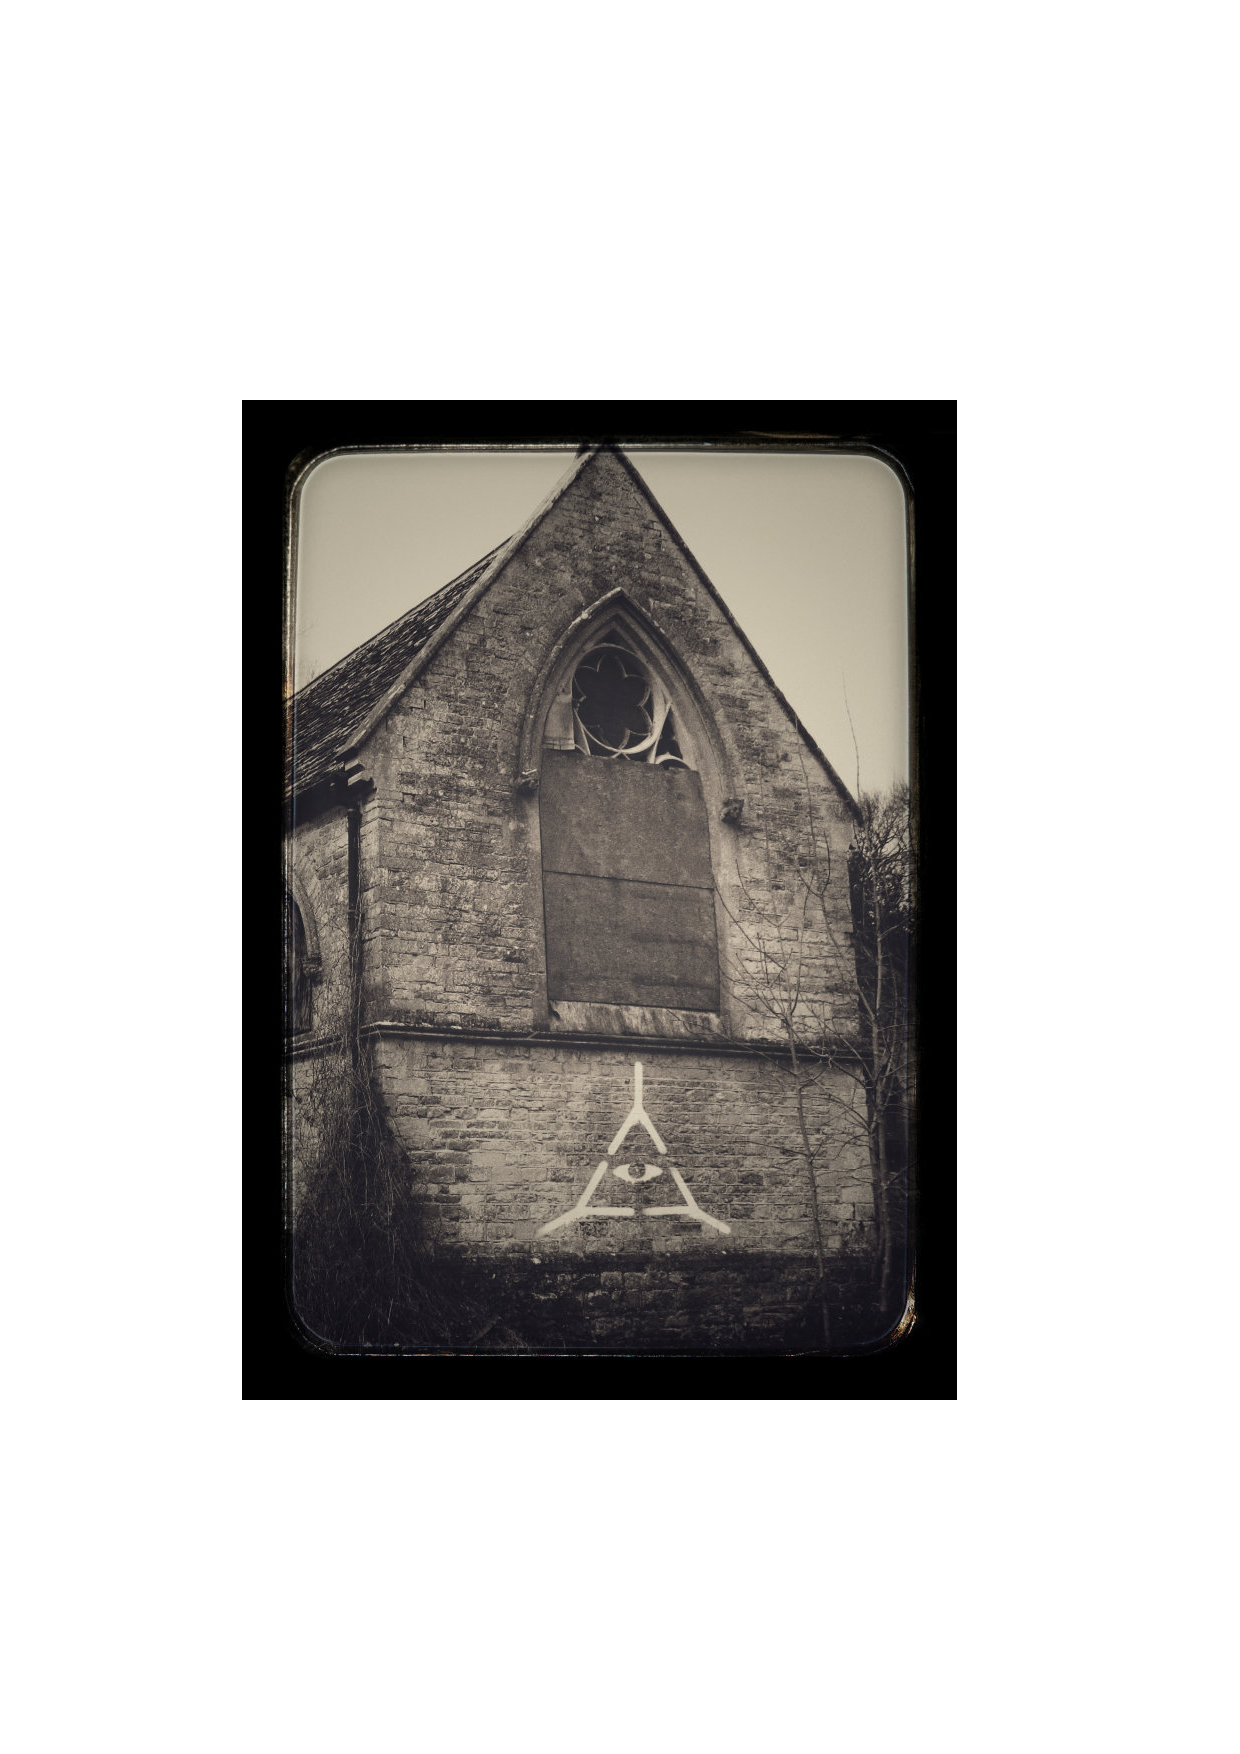
\includepdf[pages={1}, scale=1.0]{./assets/Chapel-symbol.pdf}